\chapter{System Realization}

\section{Introduction}
This final chapter focuses on the realization and testing of the HMI Stars ecosystem. We cover the Transition phase, compare the specifications with the actual system, detail the execution environment, and present functional test results and usability evaluations.

\section{Phase of Transition}
During the transition phase, the system was packaged for deployment. The web admin platform was hosted on Vercel, and the mobile client application was compiled to release builds for local client testing.

\section{Confrontation Specification vs. Realization}
Table 3.1 compares the initially specified requirements against the delivered software components to verify project completeness.

\begin{table}[H]
\centering
\caption{Confrontation table of specifications vs. realization}
\label{tab:confrontation}
\begin{tabular}{|l|p{5cm}|p{5cm}|l|}
\hline
\textbf{Req ID} & \textbf{Functional Specification} & \textbf{Realized Component} & \textbf{Status} \\
\hline
F-01 & Secure Authentication \& Reset & LoginPage \& ResetPasswordPage & Complete \\
\hline
F-02 & Employee Registry & SalariesPage list and add forms & Complete \\
\hline
F-03 & Activity pointage tracking & Monthly pointage grid calendar & Complete \\
\hline
F-04 & Leaves \& Absences requests & CongesPage form and history list & Complete \\
\hline
F-05 & Real-time message exchange & PostgreSQL Pub/Sub WebSocket chat & Complete \\
\hline
F-06 & Document storage categories & Storage buckets for KBIS, VAT, etc. & Complete \\
\hline
\end{tabular}
\end{table}

\section{Execution Environment}
The system was evaluated under the following operational environments:
*   **Admin Client (Web):** Executed on Microsoft Edge and Google Chrome browsers.
*   **Mobile Client (App):** Run on Android emulator and physical devices.
*   **Backend Server:** Supabase hosted cloud project.

\section{Application Testing}

\subsection{Demonstration of Implemented Features}
This section presents the actual user interfaces of the HMI Stars ecosystem. The system comprises two main frontends: the mobile client application used by company gérants, and the web administration platform used by the consulting enterprise's managers.

\subsubsection{Mobile Client Application Interfaces}
The mobile application provides gérants with a mobile-first interface to manage their daily social and administrative duties.

As shown in Figure \ref{fig:mobile_login_home}, the application opens with a clean welcome screen where gérants input their credentials. Upon successful authentication, they select their company profile and are redirected to the main home dashboard, which displays summary metrics and shortcuts.

\begin{figure}[H]
    \centering
    \begin{subfigure}[b]{0.32\textwidth}
        \centering
        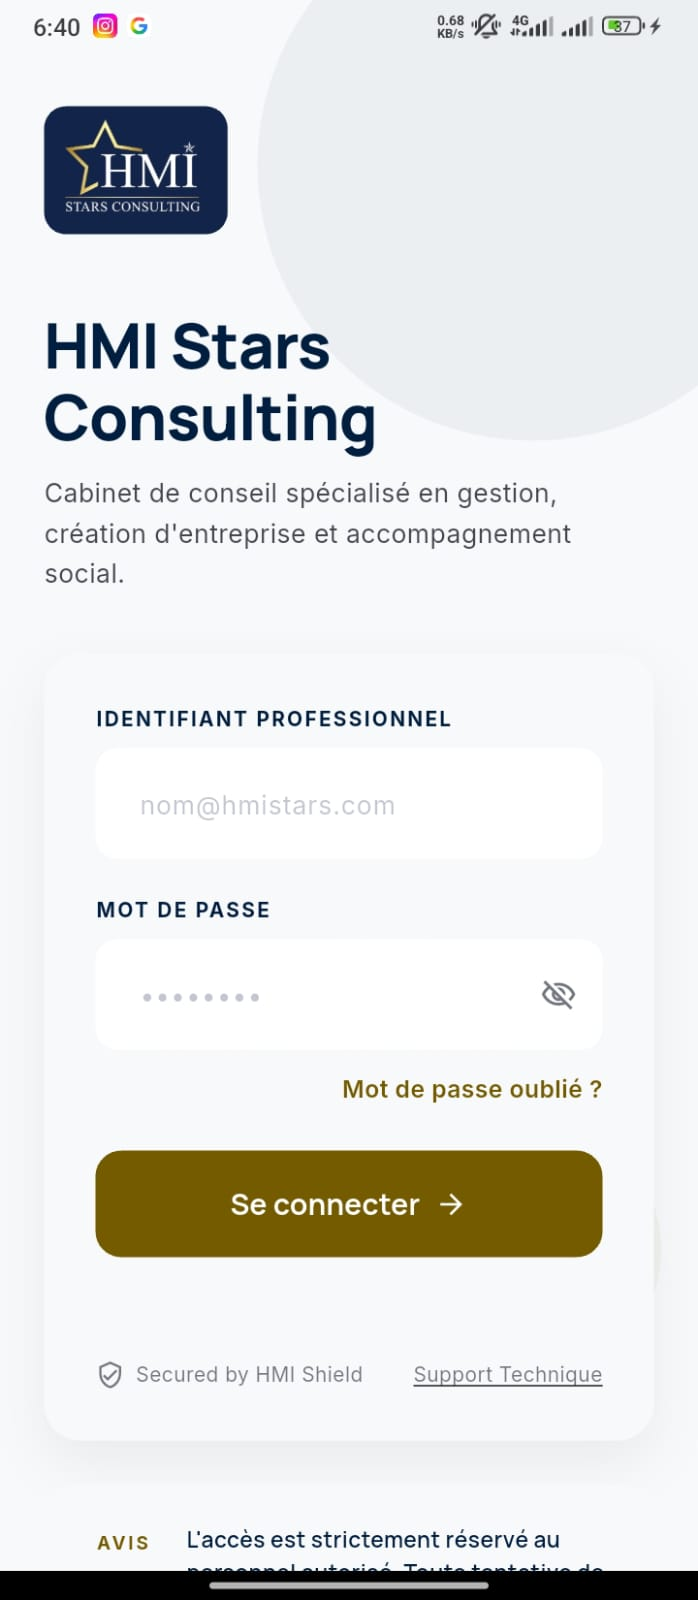
\includegraphics[width=\textwidth]{capture_application/m_welcome_screen.jpeg}
        \caption{Welcome and Login}
        \label{fig:m_login}
    \end{subfigure}
    \hfill
    \begin{subfigure}[b]{0.32\textwidth}
        \centering
        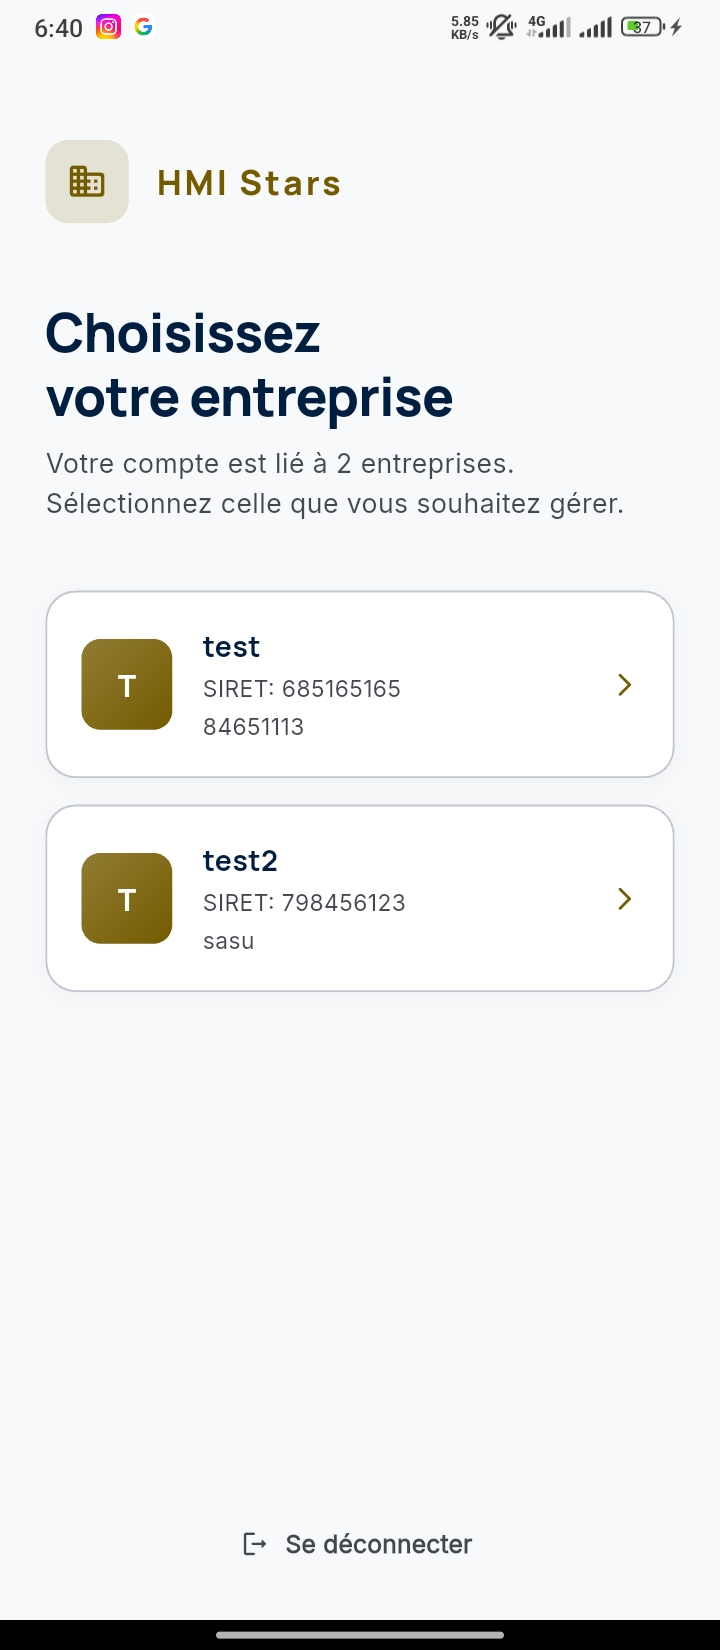
\includegraphics[width=\textwidth]{capture_application/m_choose_company.jpeg}
        \caption{Company Selection}
        \label{fig:m_select}
    \end{subfigure}
    \hfill
    \begin{subfigure}[b]{0.32\textwidth}
        \centering
        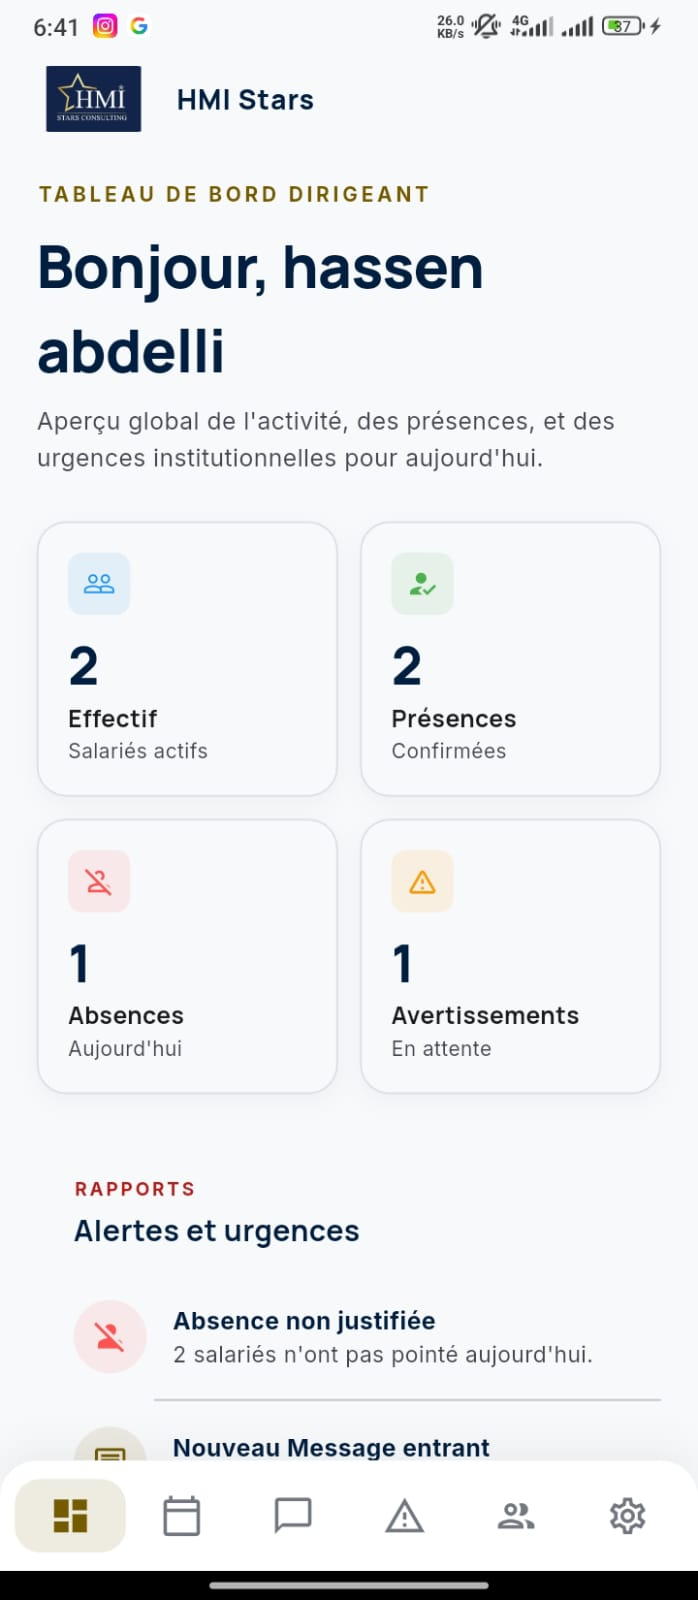
\includegraphics[width=\textwidth]{capture_application/m_home_screen.jpeg}
        \caption{Main Home Dashboard}
        \label{fig:m_home}
    \end{subfigure}
    \caption{Mobile Application - Authentication and Dashboard Interfaces}
    \label{fig:mobile_login_home}
\end{figure}

Gérants can track their employees' daily activities and register pointages. As illustrated in Figure \ref{fig:mobile_pointage}, the system provides a clean calendar-based interface where gérants can review employee status and log daily attendance.

\begin{figure}[H]
    \centering
    \begin{subfigure}[b]{0.48\textwidth}
        \centering
        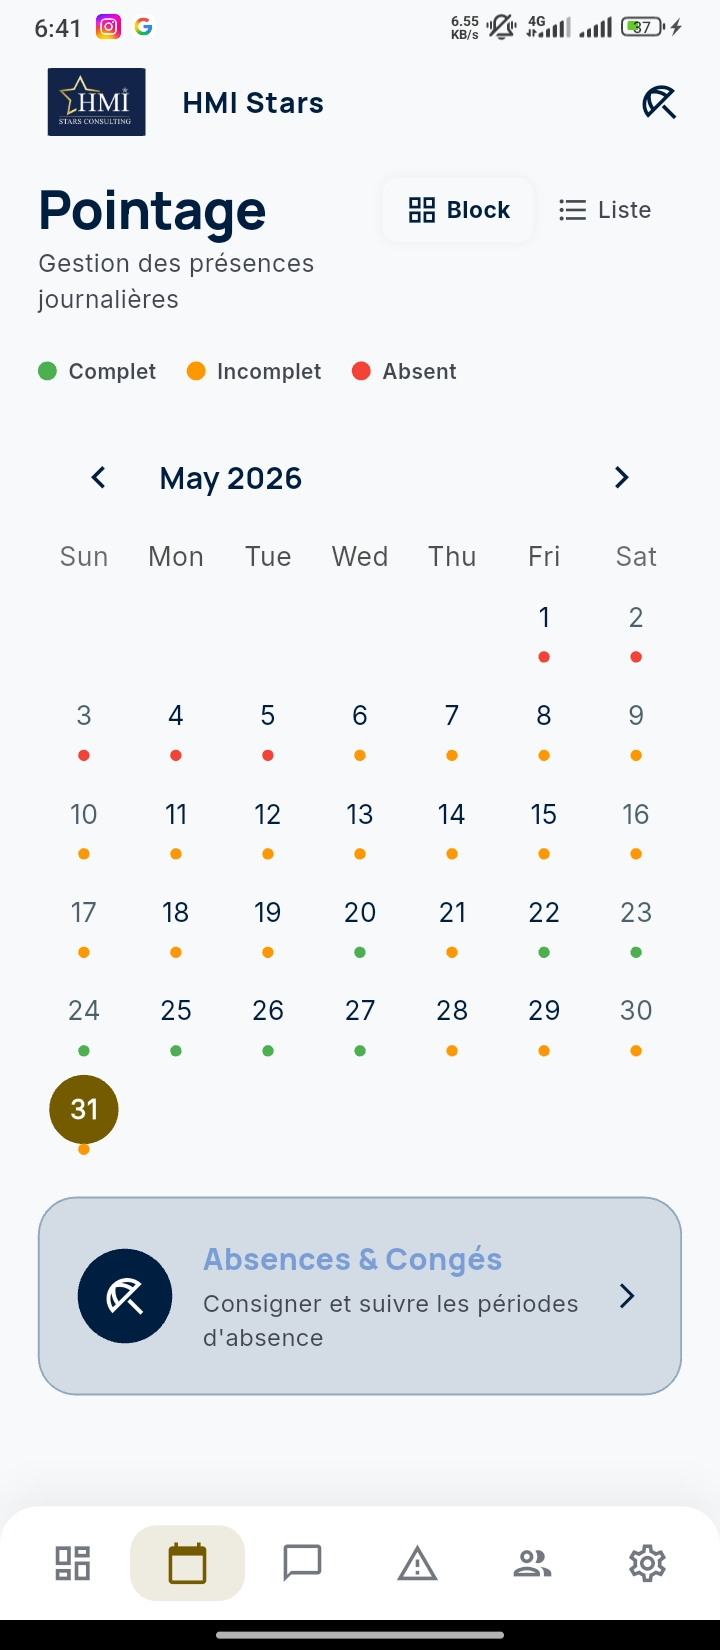
\includegraphics[width=\textwidth]{capture_application/m_pointage_cal.jpeg}
        \caption{Pointage Calendar view}
        \label{fig:m_pointage_cal}
    \end{subfigure}
    \hfill
    \begin{subfigure}[b]{0.48\textwidth}
        \centering
        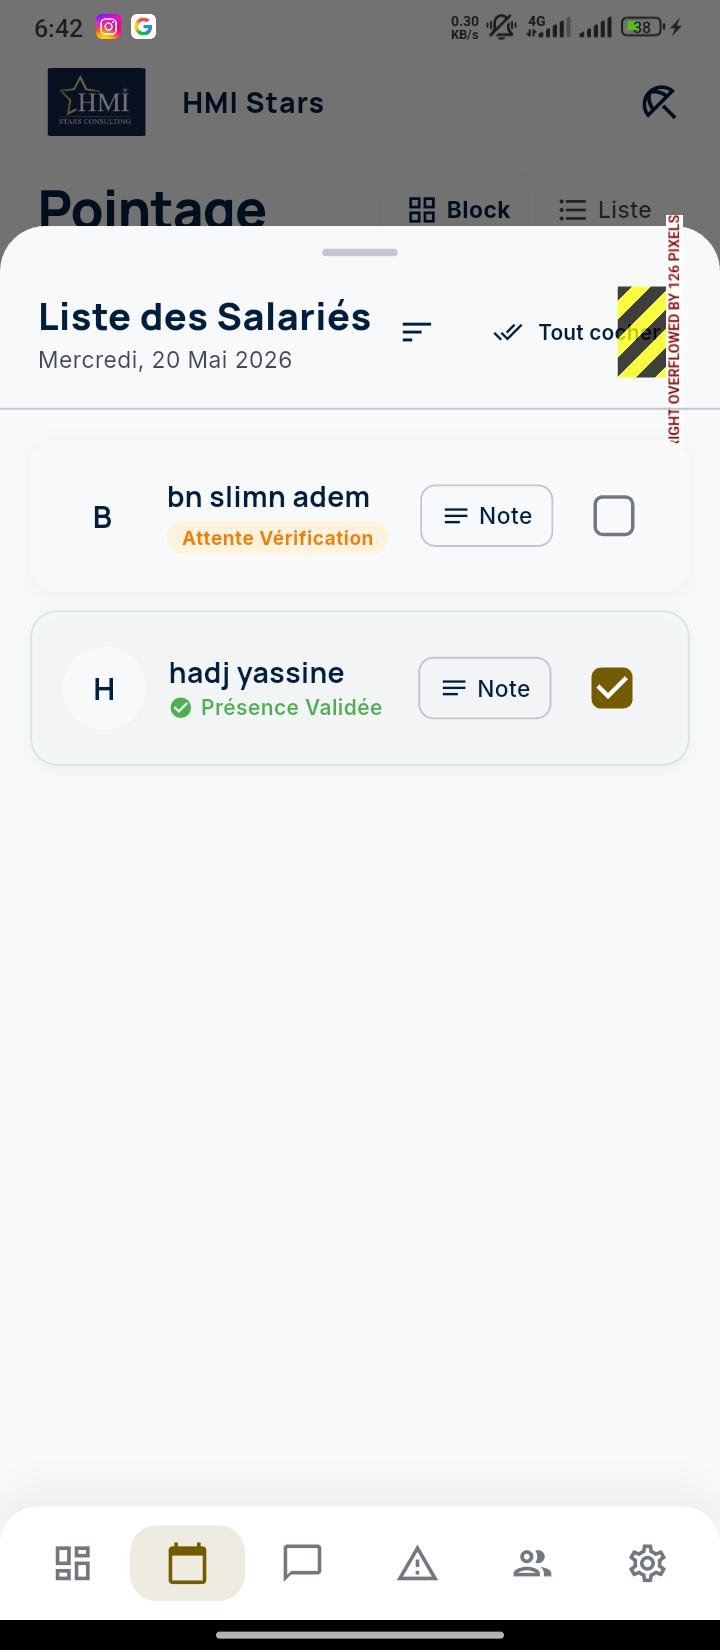
\includegraphics[width=\textwidth]{capture_application/m_employees_list.jpeg}
        \caption{Employees attendance list}
        \label{fig:m_pointage_list}
    \end{subfigure}
    \caption{Mobile Application - Daily Activity Pointage Tracking}
    \label{fig:mobile_pointage}
\end{figure}

The leaves and absences request subsystem allows gérants to declare absences and submit leave requests. Figure \ref{fig:mobile_leaves} shows the interface where requests are registered along with justifications and descriptive notes.

\begin{figure}[H]
    \centering
    \begin{subfigure}[b]{0.48\textwidth}
        \centering
        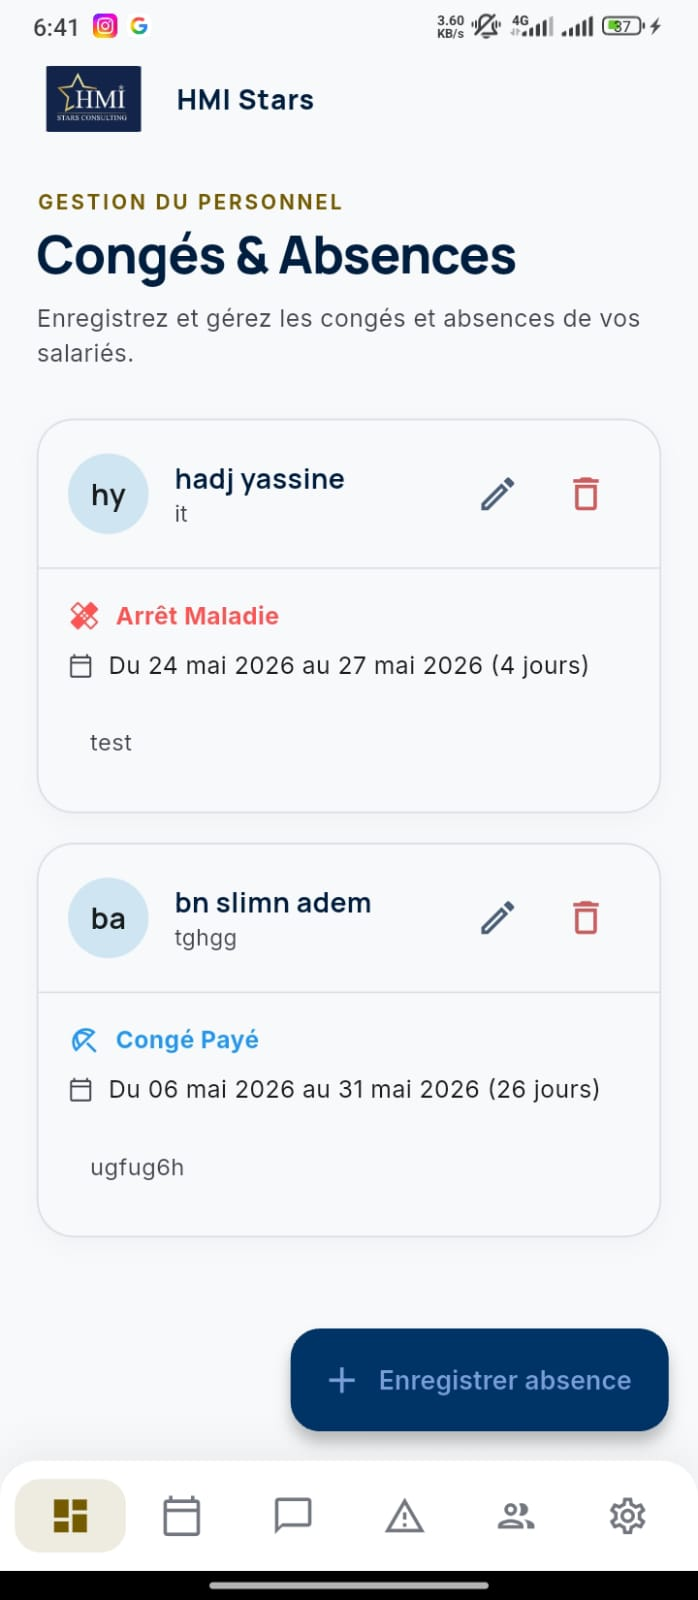
\includegraphics[width=\textwidth]{capture_application/m_leaves_list.jpeg}
        \caption{Leaves list view}
        \label{fig:m_leaves_list}
    \end{subfigure}
    \hfill
    \begin{subfigure}[b]{0.48\textwidth}
        \centering
        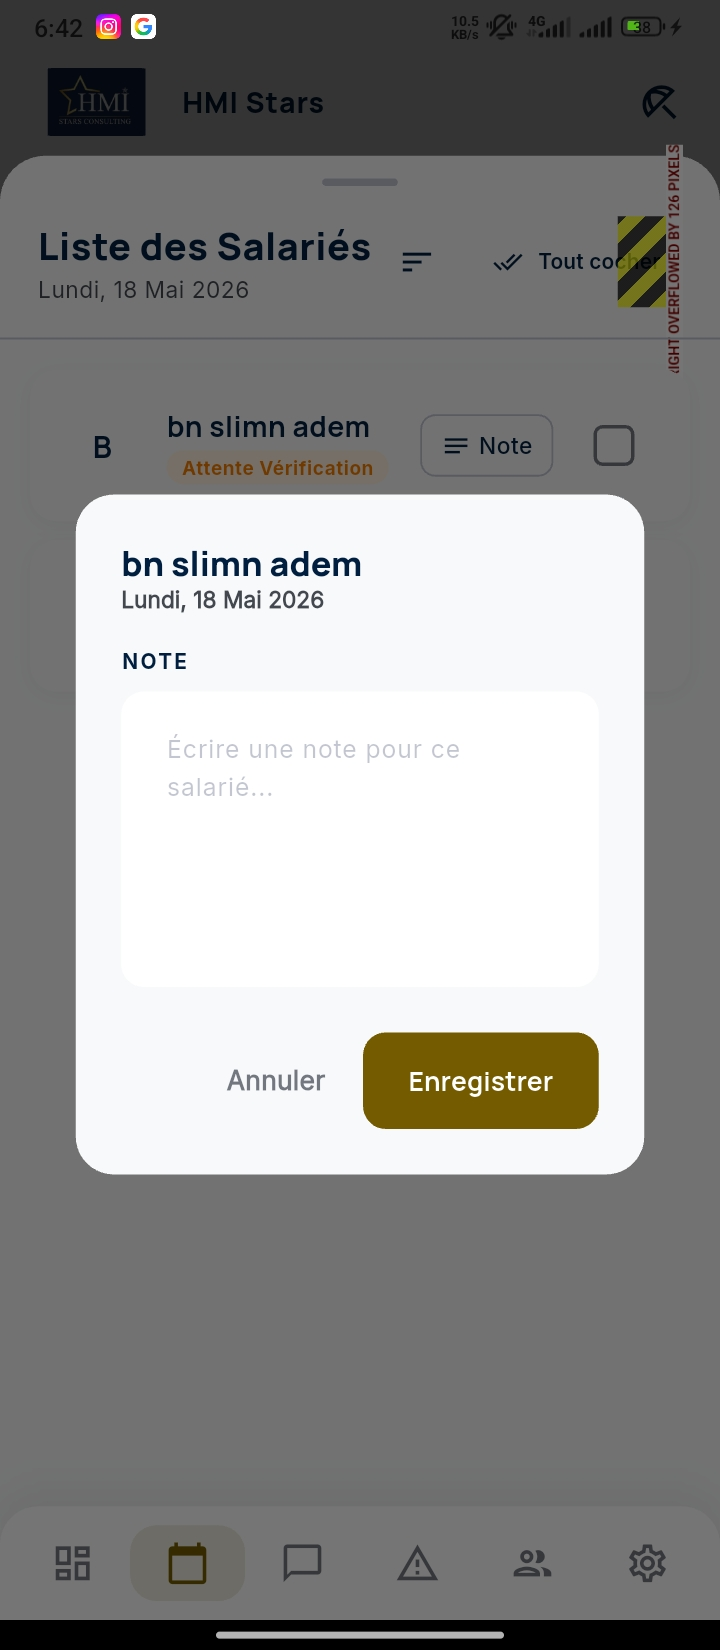
\includegraphics[width=\textwidth]{capture_application/m_absence_form.jpeg}
        \caption{Absence declaration form}
        \label{fig:m_abs_form}
    \end{subfigure}
    \caption{Mobile Application - Leaves and Absences Management}
    \label{fig:mobile_leaves}
\end{figure}

The communication channel integrates real-time chat and document sharing. Gérants can exchange messages and view all uploaded files in a dedicated file history, as displayed in Figure \ref{fig:mobile_chat}.

\begin{figure}[H]
    \centering
    \begin{subfigure}[b]{0.48\textwidth}
        \centering
        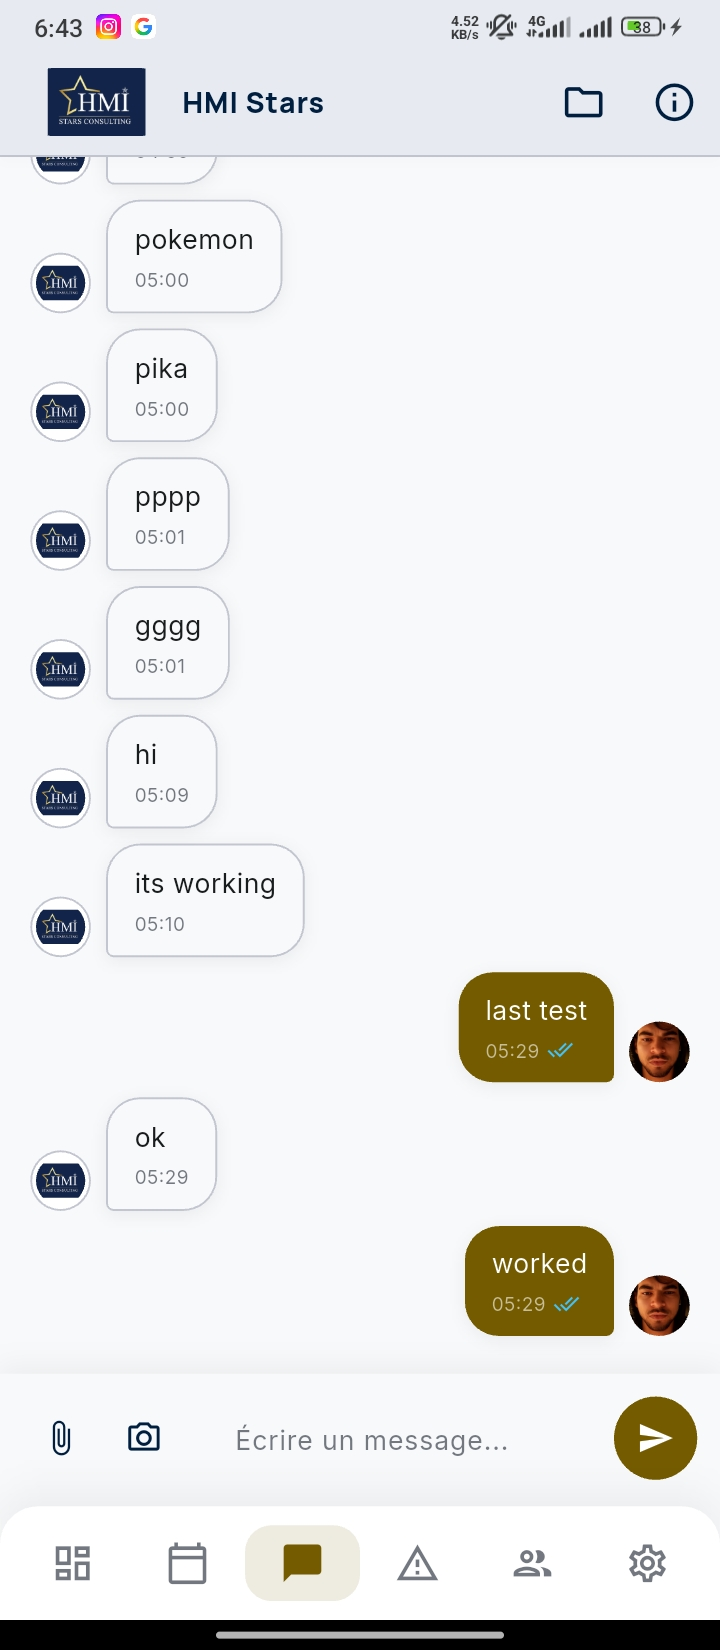
\includegraphics[width=0.9\textwidth]{capture_application/m_chat_screen.jpeg}
        \caption{Real-time chat screen}
        \label{fig:m_chat}
    \end{subfigure}
    \hfill
    \begin{subfigure}[b]{0.48\textwidth}
        \centering
        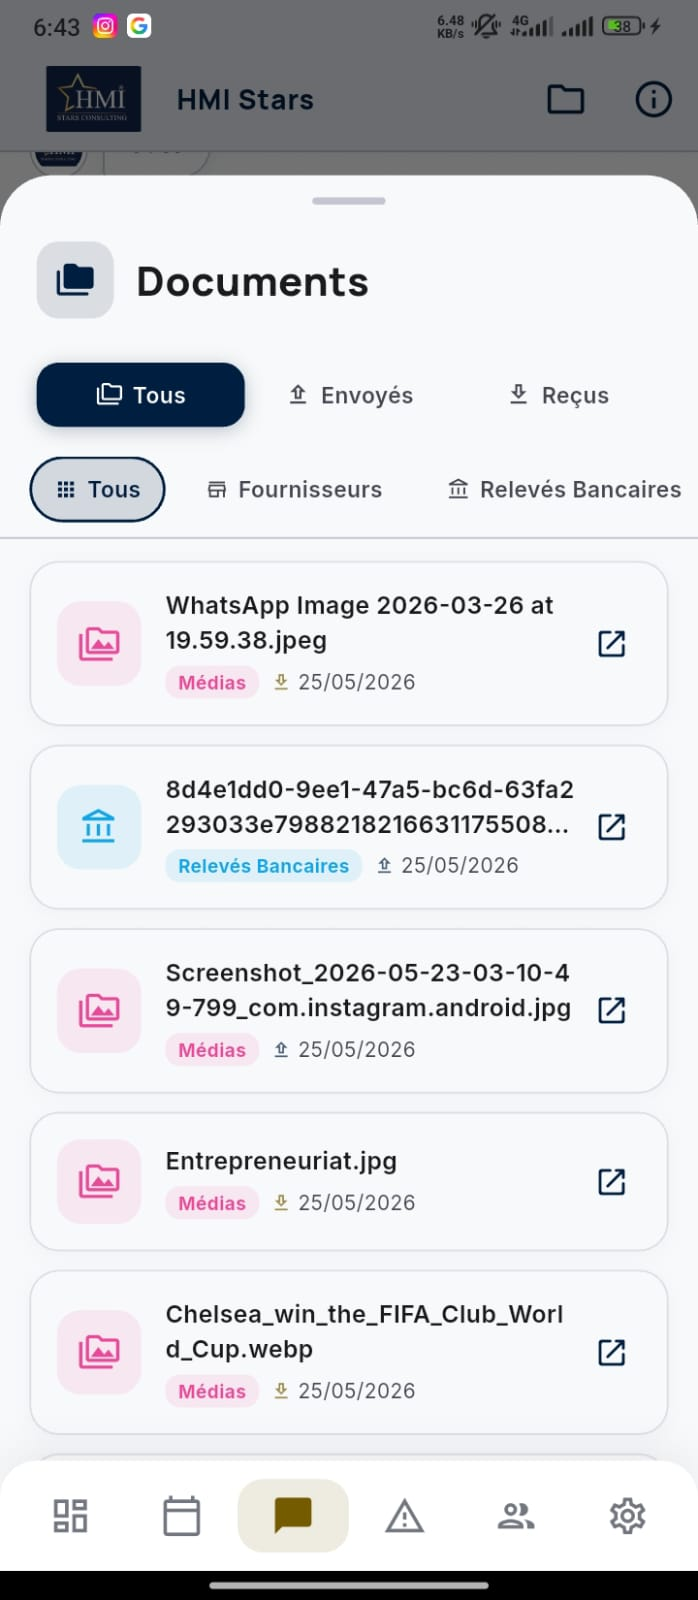
\includegraphics[width=0.9\textwidth]{capture_application/m_shared_docs.jpeg}
        \caption{Shared documents panel}
        \label{fig:m_docs}
    \end{subfigure}
    \caption{Mobile Application - Real-time Communication and Document Sharing}
    \label{fig:mobile_chat}
\end{figure}

\subsubsection{Web Administration Platform Interfaces}
The web platform allows the consulting enterprise's managers to supervise all affiliated companies and process their administrative records.

Figure \ref{fig:web_dashboard_companies} showcases the main web dashboard dashboard containing summary statistics, alongside the client companies directory showing company cards in a grid view.

\begin{figure}[H]
    \centering
    \begin{subfigure}[b]{0.48\textwidth}
        \centering
        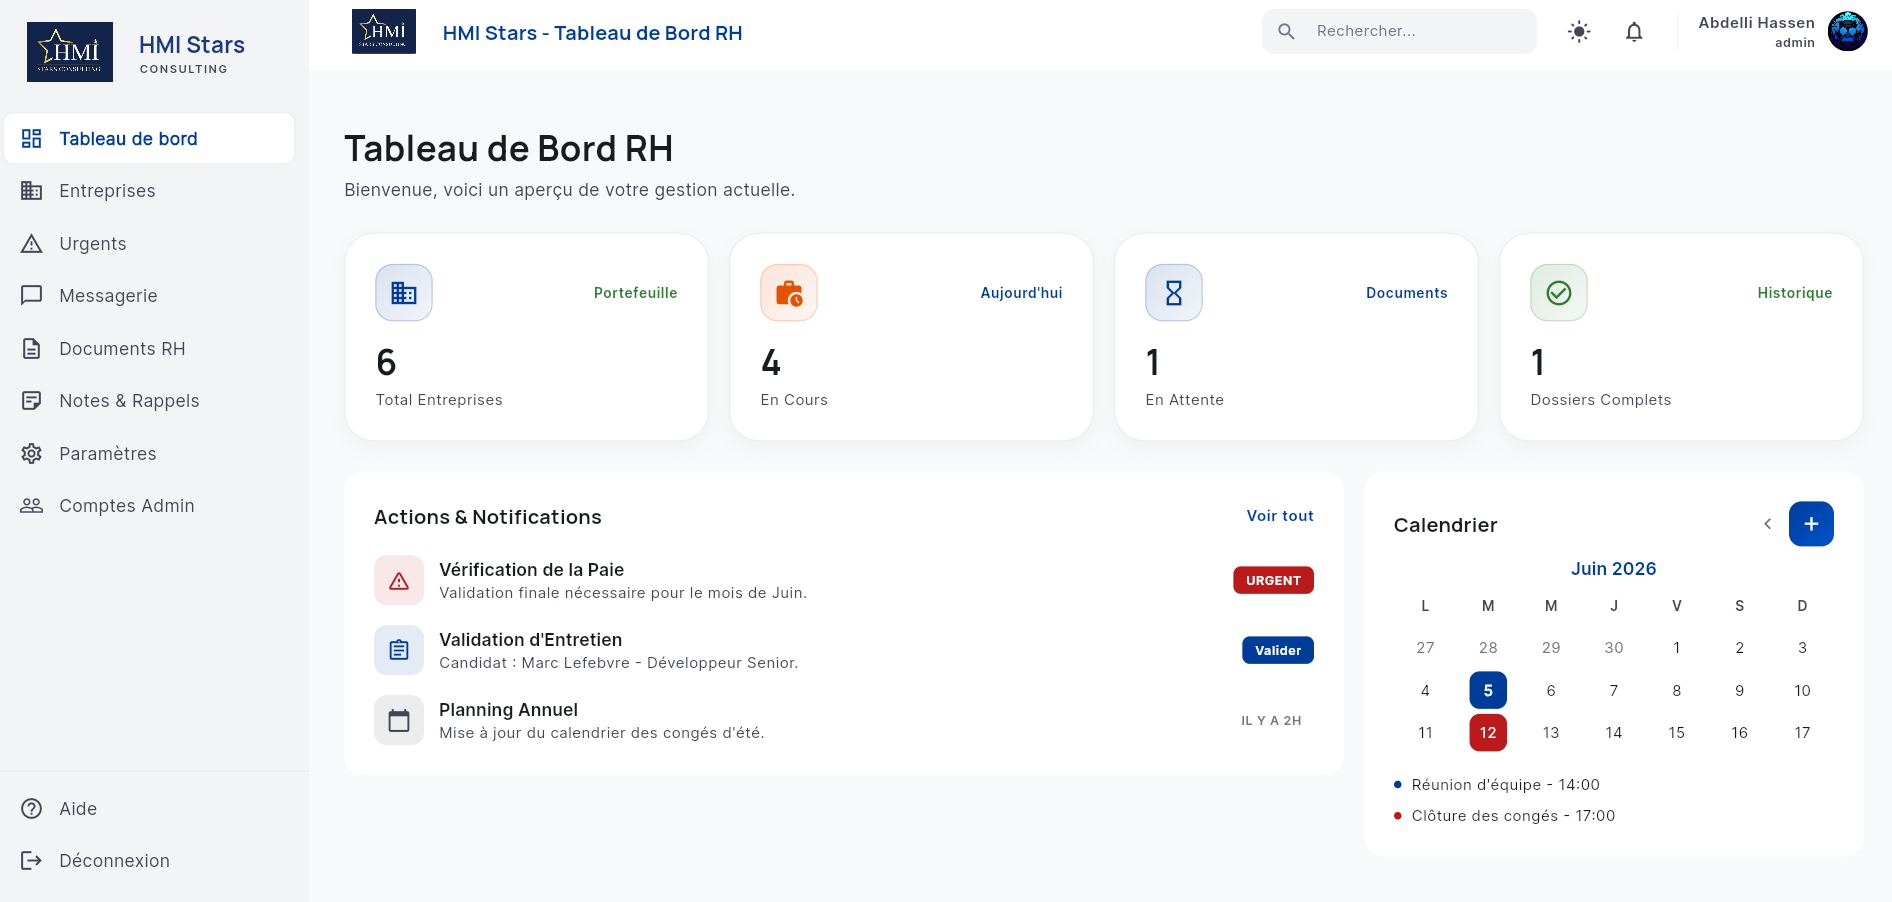
\includegraphics[width=\textwidth]{capture_platform/w_dashboard.png}
        \caption{Web Administration Dashboard}
        \label{fig:w_dash}
    \end{subfigure}
    \hfill
    \begin{subfigure}[b]{0.48\textwidth}
        \centering
        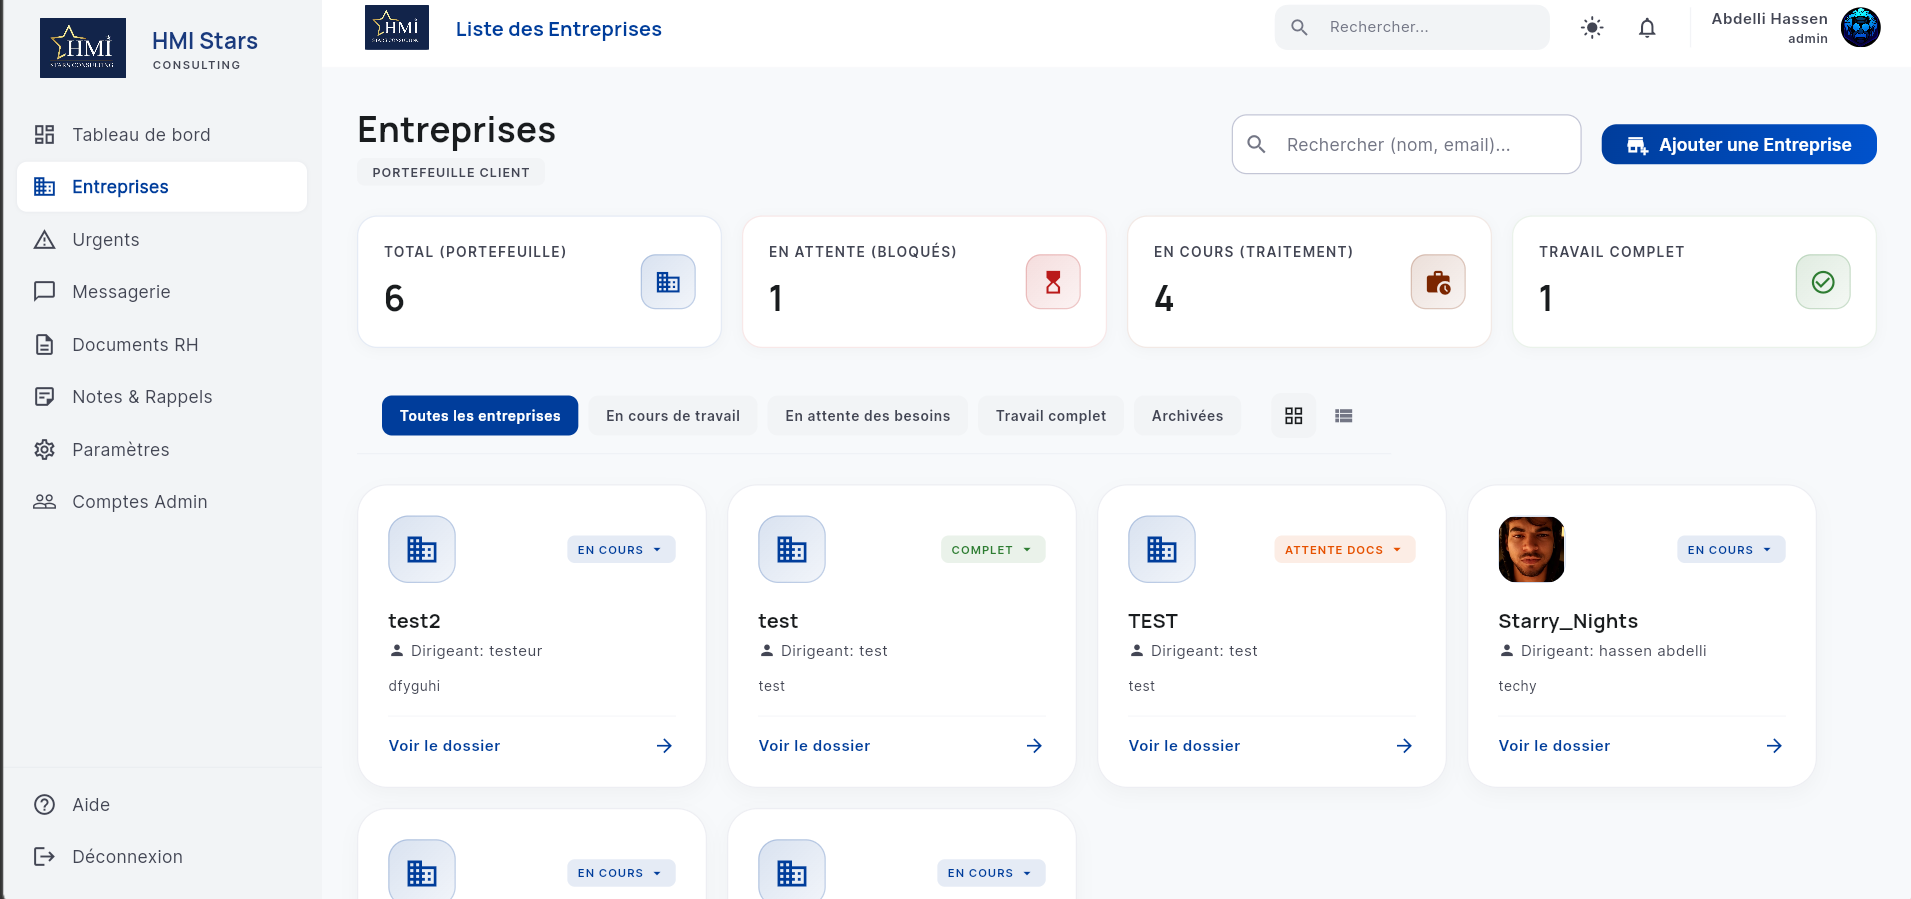
\includegraphics[width=\textwidth]{capture_platform/w_companies_grid.png}
        \caption{Client Companies Grid View}
        \label{fig:w_comp}
    \end{subfigure}
    \caption{Web Platform - Dashboard and Client Companies Directory}
    \label{fig:web_dashboard_companies}
\end{figure}

The administrator can review details of client companies and manage their employee rosters. Figure \ref{fig:web_employees} illustrates the employees list interface and the comprehensive employee details panel.

\begin{figure}[H]
    \centering
    \begin{subfigure}[b]{0.48\textwidth}
        \centering
        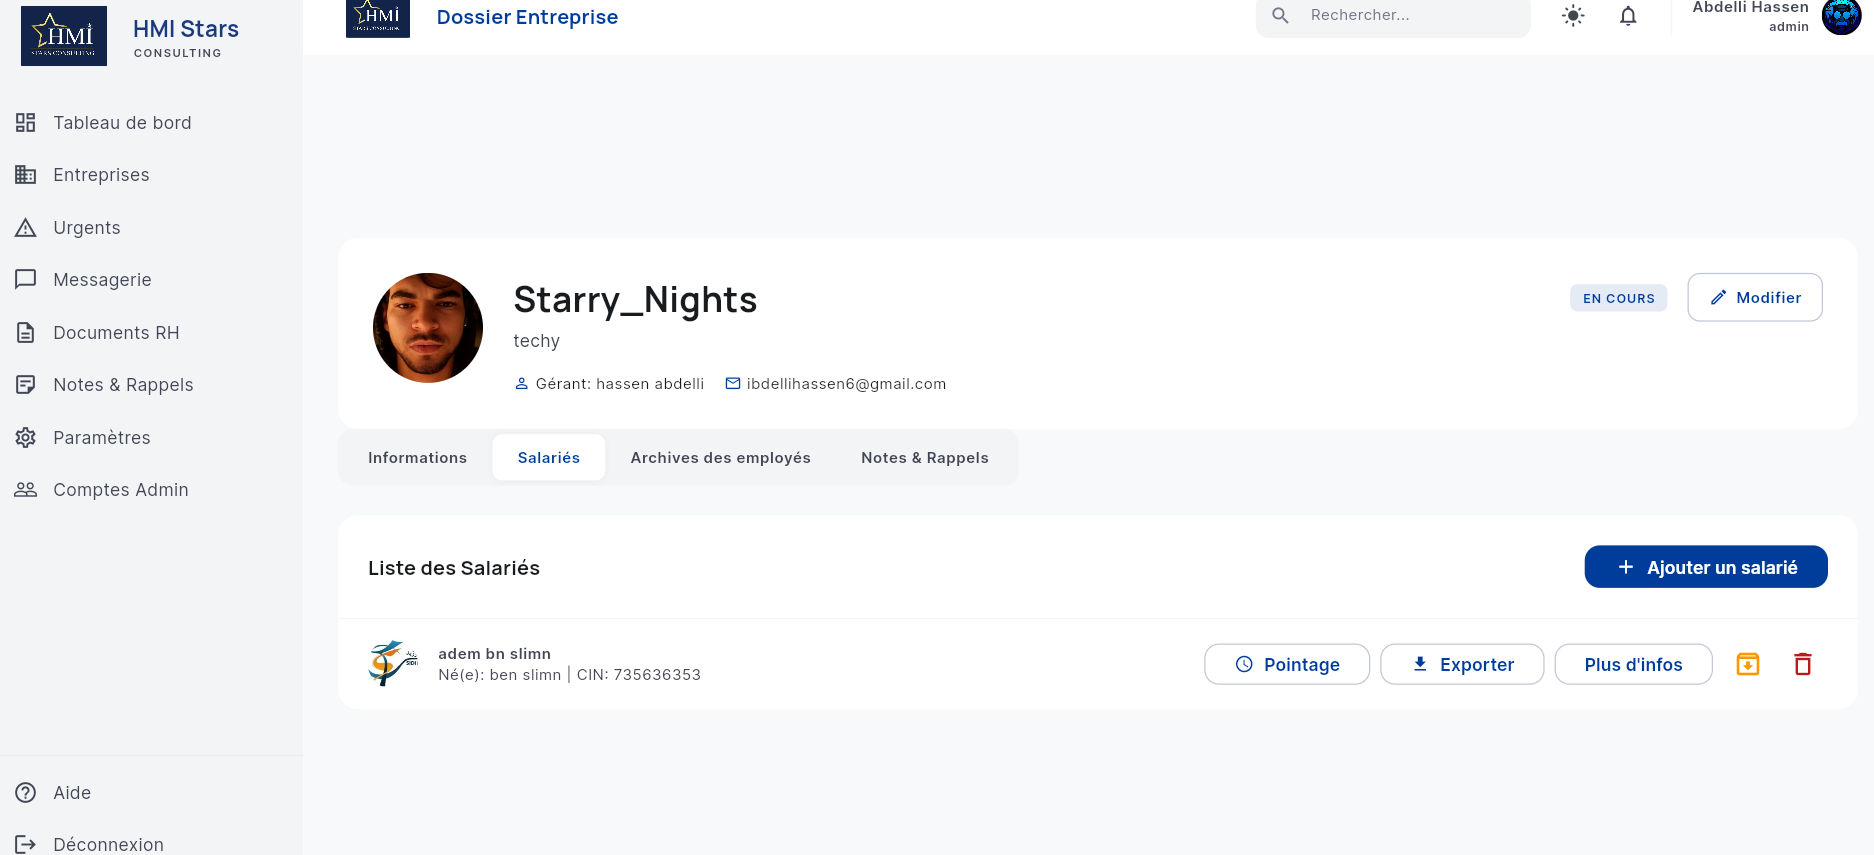
\includegraphics[width=\textwidth]{capture_platform/w_employees_list.png}
        \caption{Employees list of a client company}
        \label{fig:w_emp_list}
    \end{subfigure}
    \hfill
    \begin{subfigure}[b]{0.48\textwidth}
        \centering
        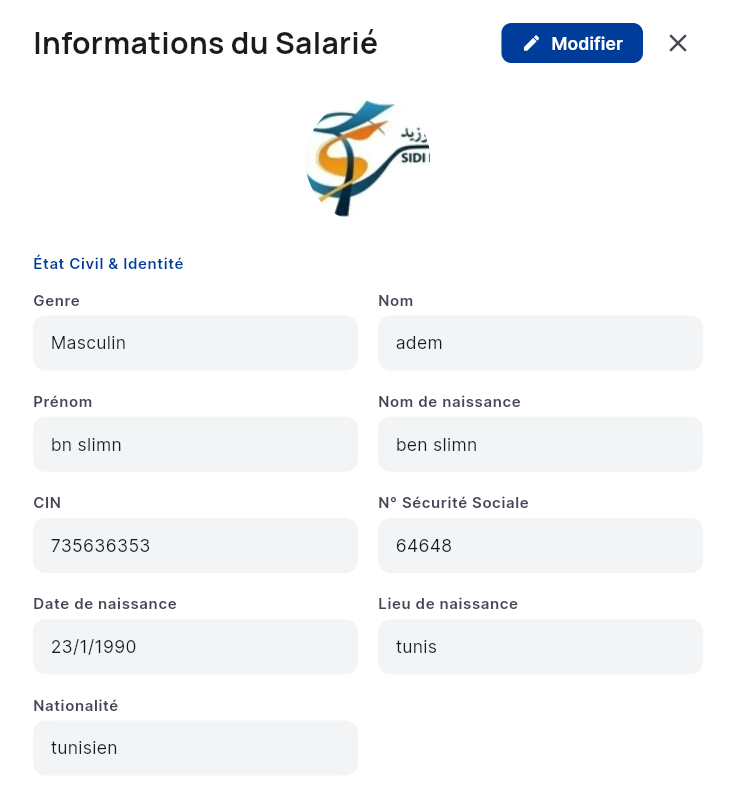
\includegraphics[width=\textwidth]{capture_platform/w_employee_details.png}
        \caption{Employee detailed information card}
        \label{fig:w_emp_card}
    \end{subfigure}
    \caption{Web Platform - Employee Management Interfaces}
    \label{fig:web_employees}
\end{figure}

The real-time messaging interface on the web is synchronized with the mobile app. Administrators can exchange messages, download documents, and filter file types, as shown in Figure \ref{fig:web_messaging}.

\begin{figure}[H]
    \centering
    \begin{subfigure}[b]{0.48\textwidth}
        \centering
        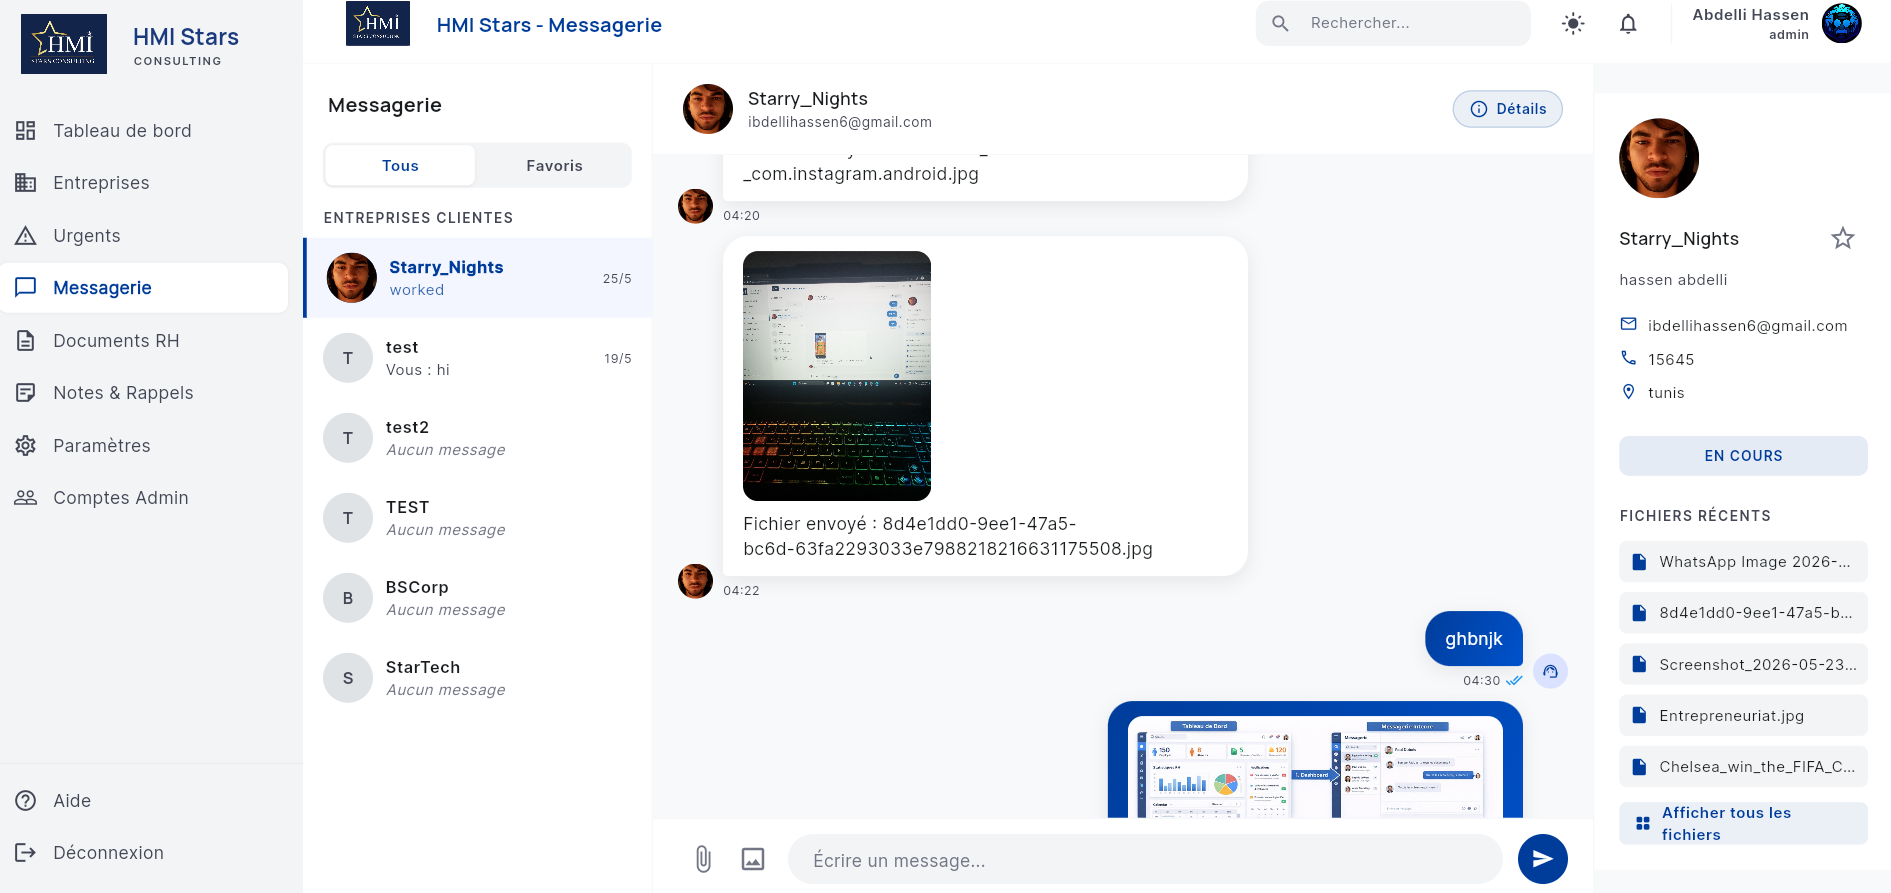
\includegraphics[width=\textwidth]{capture_platform/w_chat_workspace.png}
        \caption{Admin chat workspace}
        \label{fig:w_chat}
    \end{subfigure}
    \hfill
    \begin{subfigure}[b]{0.48\textwidth}
        \centering
        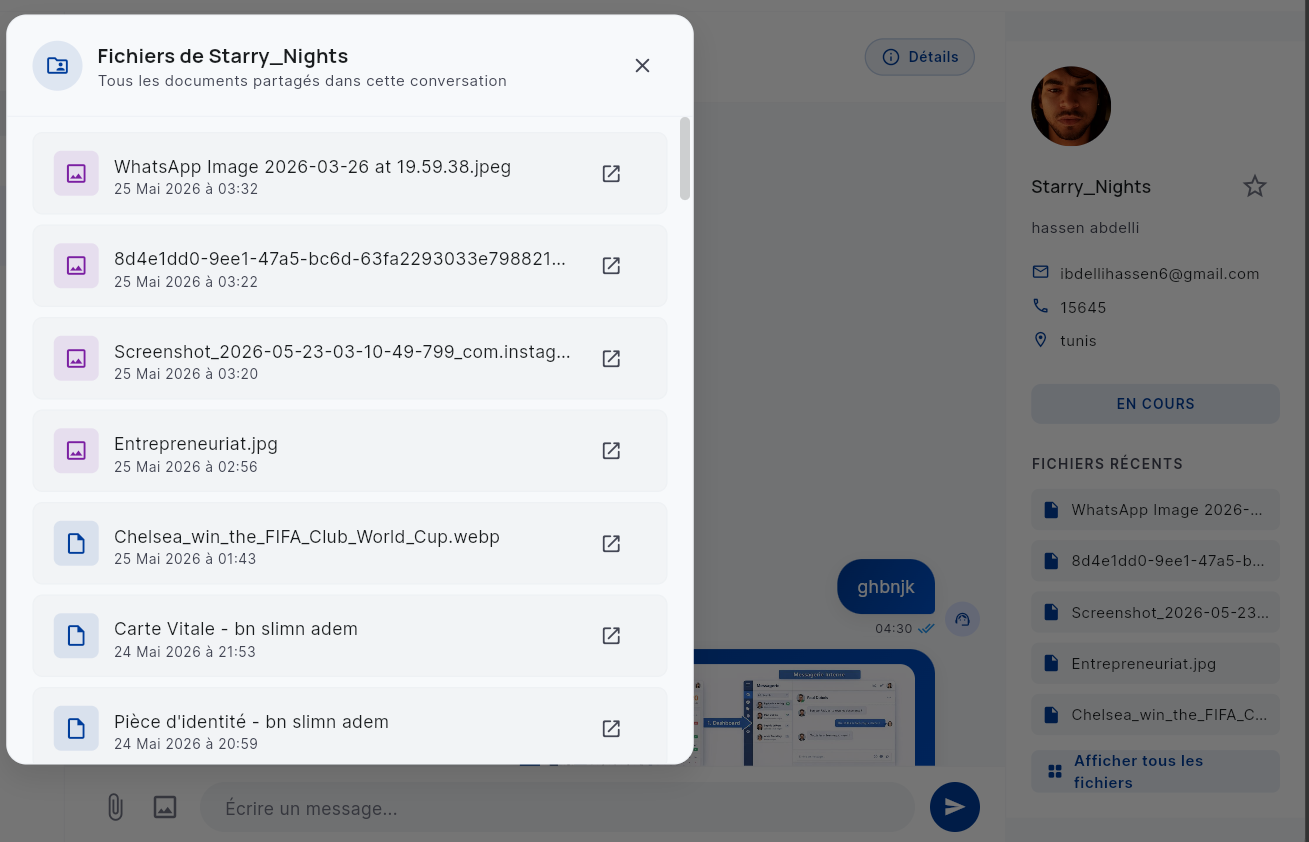
\includegraphics[width=\textwidth]{capture_platform/w_shared_files.png}
        \caption{Shared files list}
        \label{fig:w_docs}
    \end{subfigure}
    \caption{Web Platform - Real-time Messaging and File Archive}
    \label{fig:web_messaging}
\end{figure}

\subsection{Utility Evaluation}
The utility of the system was evaluated by five staff members of HMI Stars Consulting. The automated transmission of VAT and KBIS documents reduced average document collection delays from 4 days to less than 2 hours.

\subsection{Usability Evaluation}
A usability evaluation was conducted with client gérants. The average system response time for real-time messages was clocked at under 450ms. Using the Path URL routing strategy and Supabase implicit auth flow resolved the login redirect loop on web browsers, ensuring a smooth password reset process.

\section{Conclusion}
The testing and evaluation phases conenterpriseed that the HMI Stars system is stable, secure, and meets all initial project requirements. The transition phase successfully deployed the components to production environments.
